% Leistungsanalyse
% @author Tristan Ropers
%
\chapter{Evaluation}

Um die Leistung des Algorithmus und der RPC-Lösung zu bewerten wurden mehrere Experimentdurchläufe mit verschiedenen
Roboterzahlen und Zykluszeiten durchgeführt.\\

Daten zum Testsystem:
\begin{itemize}
 \item Prozessor: AMD Ryzen 7 2700X Eight-Core Processor mit 8 Kernen, 16 Threads und 3.7GHz pro Kern
 \item RAM: 16 GB Corsair DDR4 mit 2666 Mhz Taktrate
\end{itemize}

Jeder Experimentdurchlauf wurde pro Roboteranzahl mit zwei Zykluszeiten getestet, 500 Millisekunden und 800
Millisekunden. Die Schweißzeit pro Roboter wurde in der Simulation bei 150 ms angesetzt.

\clearpage

\section{Experimentdurchläufe}

\subsection{Experimentdurchlauf mit drei Robotern}

\begin{figure}[h]
 \begin{subfigure}{.5\textwidth}
  \centering
  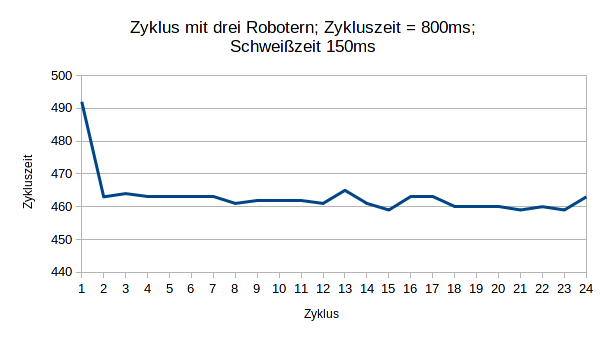
\includegraphics[width=\linewidth]{../evaluation_results/3_800.png}
  \caption{Durchlauf mit drei Robotern und \newline 800ms Zykluszeit}
  \label{fig:eval_3_800}
 \end{subfigure}
 \begin{subfigure}{.5\textwidth}
  \centering
  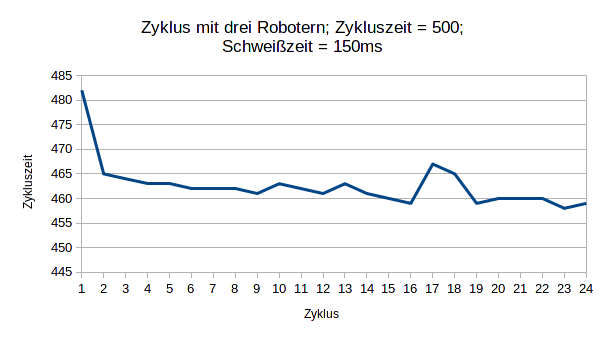
\includegraphics[width=\linewidth]{../evaluation_results/3_500.png}
  \caption{Durchlauf mit drei Robotern und \newline 500ms Zykluszeit}
  \label{fig:eval_3_500}
 \end{subfigure}
 \caption{Experimentdurchlauf mit drei Robotern}
 \label{fig:eval_3}
\end{figure}

Im ersten Durchlauf \ref{fig:eval_3} mit jeweils 800ms \ref{fig:eval_3_800} und 500ms \ref{fig:eval_3_500}
Zykluszeit ist zu erkennen, dass der erste Zyklus länger braucht als die darauf folgenden. Dies liegt daran,
dass am Anfang durch die Registrierung der Roboter und der Wahl des ersten Koordinators mehr Nachrichten
verarbeitet werden müssen als später im Durchlauf. Die Zykluszeit pendelt sich nach dem ersten Zyklus bei
einem Durchschnittswert von 461ms ein. Wenn man die Schweißzeit pro Roboter rausrechnet (150ms pro Roboter,
also 450ms pro Zyklus) kommt man auf 11ms reine Bearbeitungszeit des Algorithmus.

\clearpage

\subsection{Experimentdurchlauf mit vier Robotern}
\label{lamport_problem}

\begin{figure}[h]
 \begin{subfigure}{.5\textwidth}
  \centering
  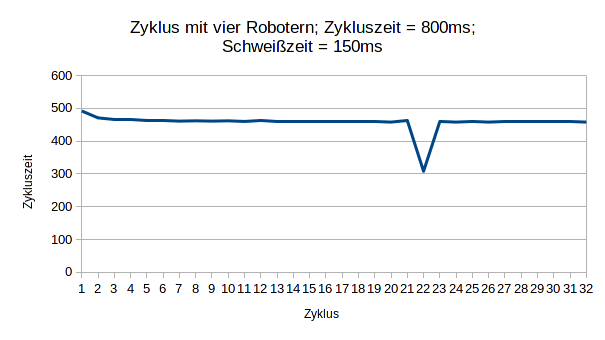
\includegraphics[width=\linewidth]{../evaluation_results/4_800.png}
  \caption{Durchlauf mit vier Robotern und \newline 800ms Zykluszeit}
  \label{fig:eval_4_800}
 \end{subfigure}
 \begin{subfigure}{.5\textwidth}
  \centering
  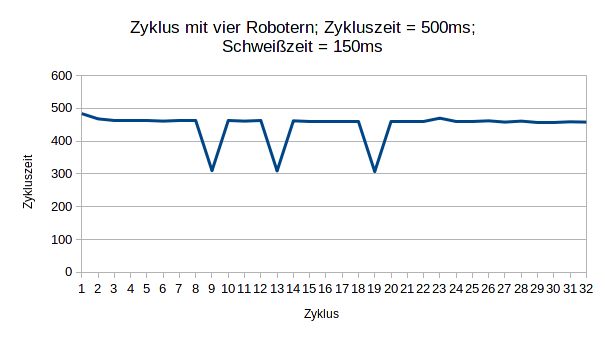
\includegraphics[width=\linewidth]{../evaluation_results/4_500.png}
  \caption{Durchlauf mit vier Robotern und \newline 500ms Zykluszeit}
  \label{fig:eval_4_500}
 \end{subfigure}
 \caption{Experimentdurchlauf mit vier Robotern}
 \label{fig:eval_4}
\end{figure}

Ein Experimentdurchlauf mit vier Robotern \ref{fig:eval_4} unterscheidet sich nicht von einem mit drei Robotern
hinsichtlich Zykluszeiten. Eine Auffälligkeit existiert jedoch in Form von auffällig kurzen Zykluszeiten (siehe
Zyklus 22 in \ref{fig:eval_4_800} oder Zyklus 9, 13 und 20 in \ref{fig:eval_4_500}. Dies ist darauf zurückzuführen,
dass alle Roboter gleichzeitig versuchen per Lamport Zugriff auf die Ressource zu erhalten. Wenn nun ein ein 
Prozess bei allen anderen den Zugriff erbittet und niemand in der Zeit selbst einen Zugriff auf die Ressource
erbittet, greift er auf die Ressource zu, obwohl ein anderer Prozess mit höherer ID und gleichem
Timestamp eher Zugriff auf die Ressource erhalten würde. Lamport erwartet allerdings eine klare Reihenfolge der
Events die in dem System auftreten \citep{lamport} (Erbitten der Ressource, Freigabe der Ressource).

\clearpage

\subsection{Auswirkung der Skalierung auf Zykluszeit}

\begin{figure}[h]
 \begin{subfigure}{.5\textwidth}
  \centering
  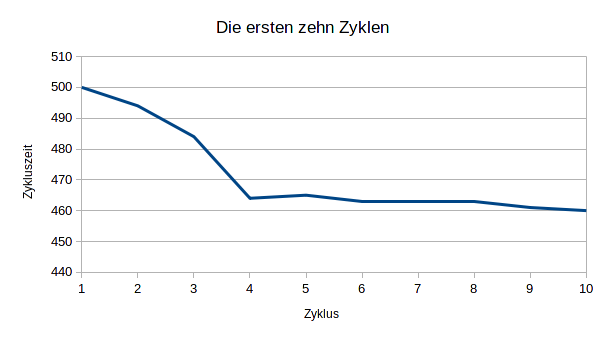
\includegraphics[width=\linewidth]{../evaluation_results/8_500_first10.png}
  \caption{Die ersten 10 Zyklen eines Durchlaufs mit 8 Robotern und 500ms Zykluszeit}
  \label{fig:eval_8_first10}
 \end{subfigure}
 \begin{subfigure}{.5\textwidth}
  \centering
  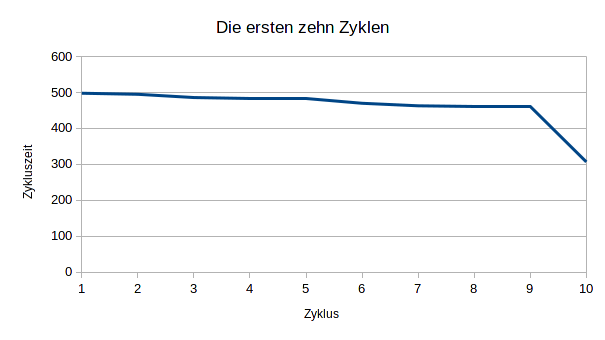
\includegraphics[width=\linewidth]{../evaluation_results/16_500_first10.png}
  \caption{Die ersten 10 Zyklen eines Durchlaufs mit 16 Robotern und 500ms Zykluszeit}
  \label{fig:eval_16_first10}
 \end{subfigure}
 \caption{Experimentdurchlauf mit 8 und 16 Robotern}
 \label{fig:eval_8_16_first10}
\end{figure}

In \ref{fig:eval_8_16_first10} zu erkennen hat die unterschiedliche Problemgröße der Durchläufe einen Einfluss
auf die Zykluszeiten am Anfang des Experiments. Während bei 8 Robotern die Zykluszeit bereits ab dem 4. Zyklus
(\ref{fig:eval_8_first10}) sich auf dem Durchschnittswert von 461ms einpendelt braucht es bei 16 Robotern
10 Zyklen (\ref{fig:eval_16_first10}). Die mit jedem zusätzlich teilnehmenden Roboter steigende
Nachrichtenkomplexität sorgt für diese anfangs höheren Zykluszeiten. Es melden sich mehr Roboter im System an
demnach steigt auch die Zahl der Registrierungsnachrichten.

